\section{Logs de Ejecución y Evidencia de Pruebas Unitarias}
\label{anexo:logs}

Para validar de forma estricta la implementación matemática y lógica del estándar GOST R 34.10, se diseñó una batería de pruebas automatizadas utilizando JUnit 5 bajo la metodología TDD. Este enfoque garantiza que la salida de cada componente de software coincida bit a bit con los vectores de prueba oficiales.

\subsection{Resultados del Motor Aritmético (\texttt{CurveMathTest})}
Las pruebas asociadas a la suma y duplicación en la curva comprueban la correcta gestión de la inversión modular y la mitigación de sobreflujos numéricos en BigInteger.

\begin{figure}[H]
    \centering
    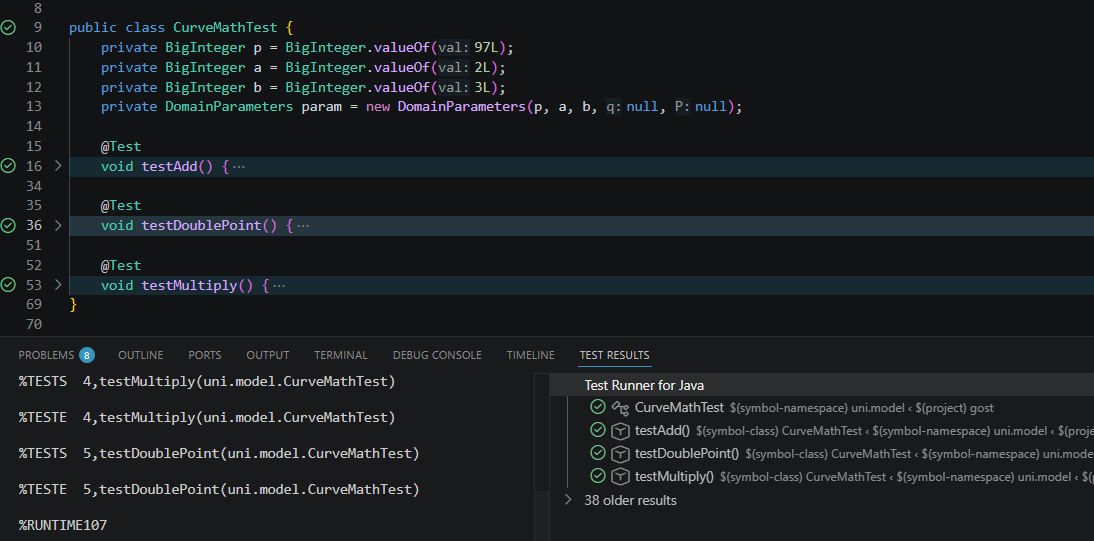
\includegraphics[width=0.85\textwidth]{imagenes/test_curvemath.png}
    \caption{Suite de pruebas unitarias ejecutadas con éxito para CurveMath.}
    \label{fig:test_curvemath}
\end{figure}

\subsection{Resultados de la Función Hash (\texttt{StreebogTest})}
Se procesaron cadenas de texto vacías, patrones repetitivos e instrucciones de prueba de la RFC 6986, validando las matrices de sustitución no lineal (\textit{S-Box}) y las transformaciones lineales de mezcla de bytes del algoritmo Streebog.

\begin{figure}[H]
    \centering
    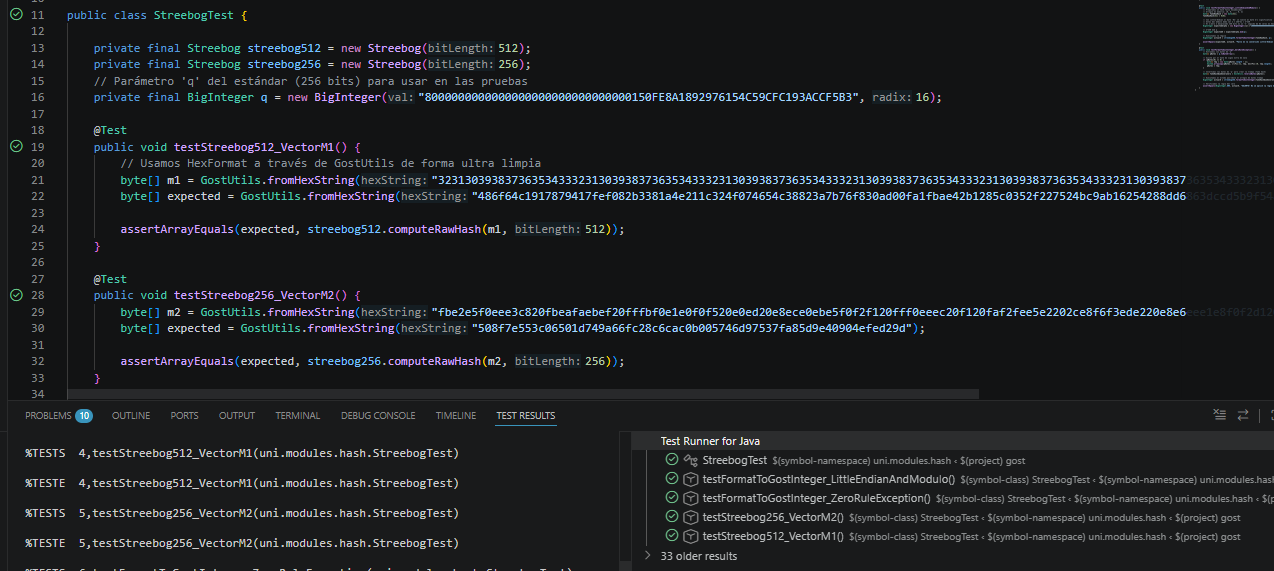
\includegraphics[width=0.85\textwidth]{imagenes/test_streebog.png}
    \caption{Verificación exitosa del vector de hash de 512 bits frente al estándar GOST R 34.11-2012.}
    \label{fig:test_streebog}
\end{figure}

\subsection{Resultados del Módulo Emisor (\texttt{SignatureGeneratorTest})}
Esta fase inyecta vectores pseudoaleatorios deterministicos para constatar que el cálculo de los componentes intermedios de la firma digital $(r, s)$ se adhiera a las especificaciones matemáticas del estándar ruso.

\begin{figure}[H]
    \centering
    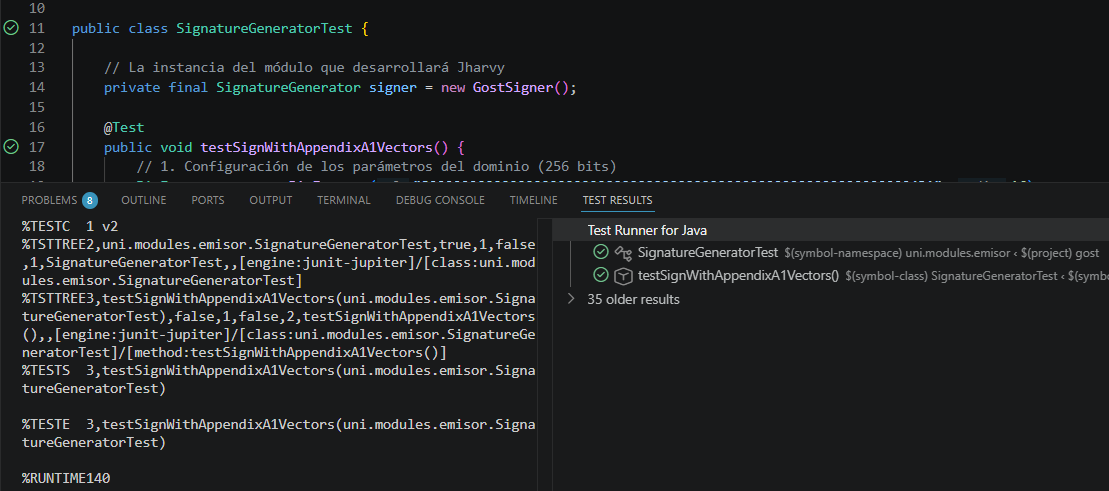
\includegraphics[width=0.85\textwidth]{imagenes/test_generator.png}
    \caption{Suite de aserciones de JUnit 5 validadas satisfactoriamente para GostSigner.}
    \label{fig:test_generator}
\end{figure}

\subsection{Resultados del Módulo Receptor (\texttt{SignatureVerifierTest})}
Las pruebas de este módulo aseguran la correcta validación de firmas auténticas y el rechazo estricto de firmas alteradas. Se verifica que la ecuación de validación reconstruya el componente $r$ original y se corrobora el manejo de casos borde, como el rechazo inmediato si los parámetros $r$ o $s$ se encuentran fuera del rango permitido ($0 < r, s < q$).

\begin{figure}[H]
    \centering
    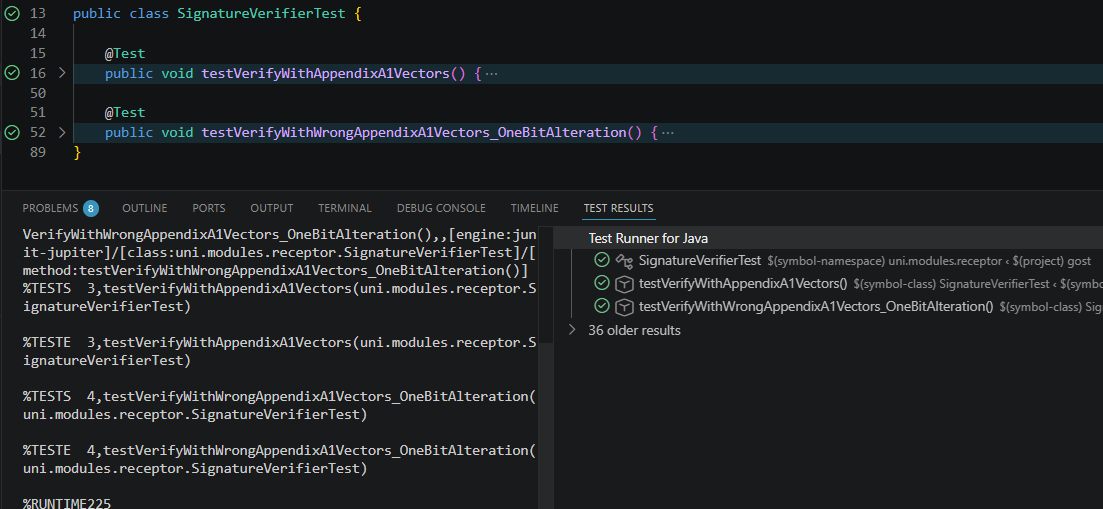
\includegraphics[width=0.85\textwidth]{imagenes/test_verifier.png}
    \caption{Resultados exitosos de las aserciones de validación de firma para GostVerifier.}
    \label{fig:test_verifier}
\end{figure}

\subsection{Log de Consola de la Aplicación Integrada}
Al compilar y ejecutar el proyecto utilizando el ciclo de vida de Maven, se genera la siguiente salida por consola, evidenciando el ciclo completo y exitoso de orquestación criptográfica:

\begin{figure}[H]
    \centering
    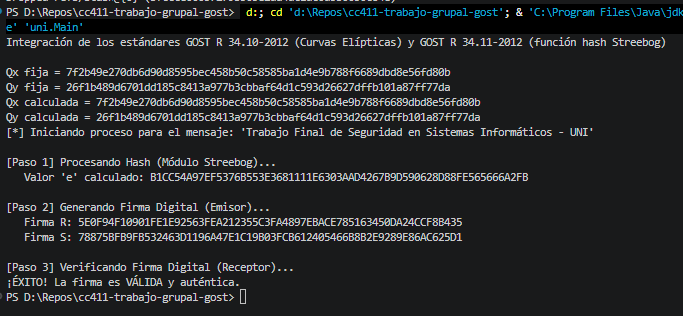
\includegraphics[width=0.85\textwidth]{imagenes/console_log.png}
    \caption{Captura de la salida estándar del sistema orquestador ejecutado en el entorno local.}
    \label{fig:console_log}
\end{figure}